\documentclass[mathserif]{beamer}

\usepackage{multicol}
\usepackage{beamerthemeshadow}
\usepackage{graphicx}
\usepackage{graphics}
\usepackage{pgf}
\usepackage{tikz}
\usepackage{hyperref}   % Hyperlink references and URLs
\usetikzlibrary{arrows,automata,petri,positioning}
\usepackage[latin1]{inputenc}

\title[AHOY: Slide \insertframenumber/\inserttotalframenumber]{AHOY: An event-based simulation environment}

\subtitle{Initial Presentation}

\author[Clark, Ingram, Kolakowska, \& Rosenfeld]{ 
Frank~Clark\inst{1}, Dustin~Ingram\inst{1}, Maria~Kolakowska\inst{1}, Aaron~Rosenfeld\inst{1}, William~Regli\inst{1}, Joseph~Macker\inst{2}, Michal~P\v{e}chou\v{e}k\inst{3}}

\institute{
    \inst{1}%
    Drexel University Department of Computer Science, Philadelphia PA
    \and
    \inst{2}%
    US Naval Research Laboratory Networks \& Communication Systems Branch, Washington DC
    \and
    \inst{3}%
    Czech Technical University Agent Technology Center, Prague
}

\date{\today}

\begin{document}

\frame{\titlepage} 

\frame
{
    \frametitle{Outline}
    \tableofcontents
}

\section{Motivation}

\subsection{Network Simulators}
\frame
{
    \frametitle{Background on Network Simulators}
    \begin{itemize}
        \item Used to test applications and protocols without physical hardware
        \item Mimic the properties of a physical network
        \item Virtualization of network components (nodes) allows multiple virtual nodes to run on one physical node
        \item Scale well, easy to re-configure
        \item Cost \& time effective
    \end{itemize}
}

\subsection{Agents}
\frame
{
    \frametitle{Background on Agents}
    \begin{block}{Definition}
    An \emph{intelligent agent} is software which observes and acts upon an environment and directs its activity towards achieving goals (Russell, Norvig).
    \end{block}

    \begin{itemize}
        \item Used to test agent algorithms within virtual worlds
        \item Rules define actions to be taken when beliefs
        \item Users define rule-sets for agents based on sensory information in the world
        \item Allows for large-scale simulation unfeasible in the real-world
    \end{itemize}
}

\subsection{Issues with Existing Tools}
\frame
{
    \frametitle{Existing tools}
    \textbf{Current Network Simulators}
    \begin{itemize}
        \item Designed for testing networks \& protocols, not agents 
        \item Scenarios are pre-scripted
        \item Poor event support
        \item Lack of templated agents
        \item Inability to batch process multiple executions of scenarios with varying settings
        \item Data collection non-existent or not directly supported
    \end{itemize}
    \textbf{Current Agent Frameworks}
    \begin{itemize}
        \item Communications modeled only at the application layer
        \item Lack of rich lower-level protocols
        \item Alternative approaches require physical hardware for networking
    \end{itemize}
}

\section{Implementation}

\subsection{Goals}
\frame
{
    \frametitle{Implementation Goals}
    \textbf{Bridge network simulators and agent simulators}
    \begin{itemize}
        \item Entirely event-driven
        \item Real-time
        \item Allow for human-in-the-loop interaction with agents
        \item Modular communication interface to support real networks \& communication
        \item Enable scenarios and network topologies to be easily defined
        \item Make writing custom agents extremely simple
        \item Visualization flexibility
        \item Physically distributed simulation
        \item Simple data collection
    \end{itemize}
}


\subsection{Overview}
\frame
{
    \frametitle{Overview of AHOY}
    \begin{itemize}
        \item AHOY is the realization of most of these goals
        \item Currently finished 2nd prototype iteration
        \item Supports:
        \begin{itemize}
            \item Event-Based Simulation
            \item Decoupled Visualization
            \item Scenario Setup \& Creation
            \item Scaled Distribution
            \item Batch Experimentation \& Data Collection
        \end{itemize}
    \end{itemize}
}

\frame
{
    \frametitle{Architecture}
    \begin{center}
        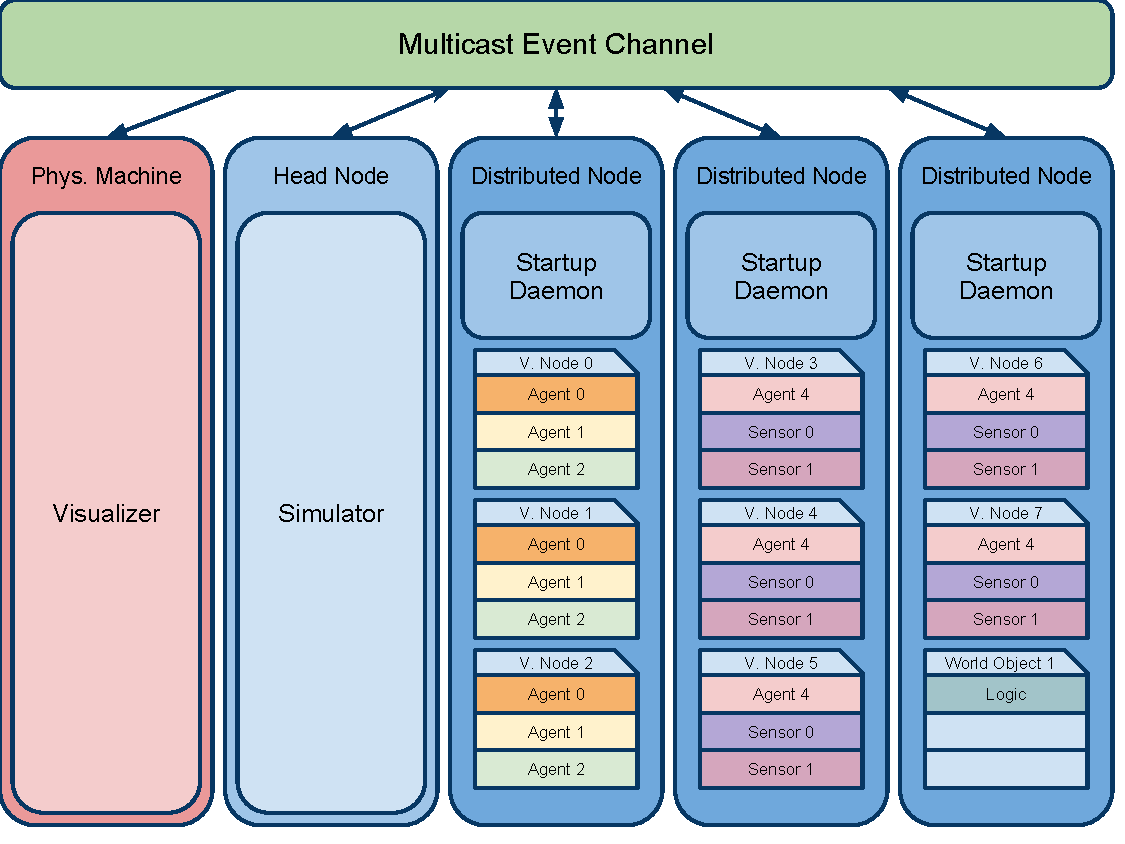
\includegraphics[scale=.4]{arch.pdf}
    \end{center}
}

\frame
{
    \frametitle{Event-Based Simulation}
    \textbf{}
    \begin{itemize}
        \item
    \end{itemize}
}


\subsection{Visualization}
\frame
{
    \frametitle{Decoupled Visualization}
    \textbf{Visualizing the Simulation}
    \begin{itemize}
        \item Monitoring the multicast event channel produces raw event data
        \item This occurs simultaneously with the execution of an experiment
        \item Any visualizer can interpret these events to produce their own visualization
        \item Completely separated from the simulator
    \end{itemize}
}

\subsection{Scenarios}
\frame
{
    \frametitle{Scenario Setup \& Creation}
    \textbf{Using a ``Programming'' Interface}
    \begin{itemize}
        \item Each of the following are defined purely in Python:
        \begin{itemize}
            \item Agent Software
            \item Network Topologies
            \item Sensor Functions
            \item World Objects
        \end{itemize}
        \item These definitions are then interpreted by the simulator to set up the experiment \& to define the 
    \end{itemize}

}

\subsection{Distribution}
\frame
{
    \frametitle{Scaled Distribution}
    \textbf{Distribution of Virtual Nodes}
    \begin{itemize}
        \item Simple to distribute: everything is an event
        \item All events are broadcast over a common event channel
        \item Agents are started on multiple physical machines
        \item Synchronization of simulation-time across physical machines may prove difficult, especially with integration of NS3; possible issues with human-in-the-loop
    \end{itemize}
}

\subsection{Experimentation}
\frame
{
    \frametitle{Batch Experimentation}
    \textbf{Running Multiple Experiments \& Collecting Data}
    \begin{itemize}
        \item Collect data from each experiment
        \item Provide tabulated results of high level metrics
        \item API to allows agents to output low-level, specific information
    \end{itemize}
}

\end{document}
